\chapter{Géométrie élémentaire du plan}
\label{chap:geomplan}
\minitoc
\minilof
\minilot
\section{Modes de repérage dans le plan}
\label{sec:modederep}
Soit $\P$ le plan géométrique euclidien. On suppose que $\P$ est muni d'un repère $\Rep=(O,\vi, \vj)$.
%
\subsection{Coordonnées cartésiennes}
\label{subsec:coordcart}
\begin{defdef}
  Soit $M$ un point du plan $\P$. Il existe un unique couple de réels $(x,y)$ tel que $\vect{OM}=x\vi+y\vj$. On appelle ce couple les coordonnées cartésiennes de $M$ dans le repère $\Rep$. Ainsi, la donnée d'un repère cartésien permet de définir une bijection entre $\R^2$ et $\P$, ce qui permettra d'identifier ces deux ensembles. %La représentation de ce mode de repérage est donnée par la figure \ref{fig:coordcart}.
\end{defdef}
% \begin{figure}
%   \centering
%   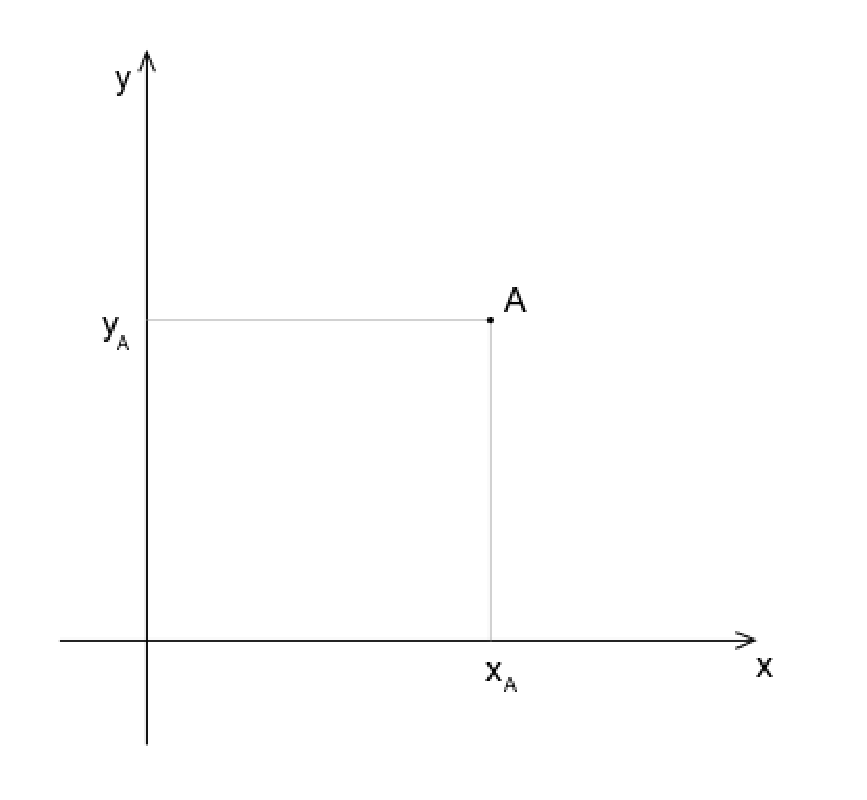
\includegraphics[scale=0.5]{coordcartesienne.eps}
%   \caption{Représentation garphique des coordonnées cartésiennes}
%   \label{fig:coordcart}
% \end{figure}
%
\subsection{Coordonnées polaires}
\label{subsec:coordpol}
  On suppose ici que $\Rep$ est un repère orthonormal direct. Pour tout réel $\theta$, on définit le vecteur $\vu_\theta$ par $\vu_\theta=\cos\theta\vi+\sin\theta\vj$. C'est l'unique vecteur $\vu$ tel que $\norme{\vu}=1$ et $\congru{(\vi,\vu)}{\theta}{2\pi}$.
\begin{defdef}
  Soit $M$ un point du plan $\P$. On dit que $(\rho,\theta)$ est un \emph{système de coordonnées polaires}~\footnote{abrégé en s.c.p.} de $M$ dans $\Rep$ si $\vect{OM}=\rho\vu_\theta$.
\end{defdef}
%
Si le point $M$ est l'origine du repère $O$ alors $(\rho,\theta)$ est un s.c.p.\ de $M$ si et seulement si $\rho=0$ et l'angle $\theta$ est quelconque. Si $M$ n'est pas l'origine du repère alors $(\rho,\theta)$ est un s.c.p.\ de $M$ si et seulement si $\rho=OM$ et $\congru{(\vi,\vu)}{\theta}{2\pi}$ ou si $\rho=-OM$ et $\congru{(\vi,\vu)+\pi}{\theta}{2\pi}$. Pour un même point, il existe une infinité de s.c.p.\ possibles. Par contre un s.c.p.\ définit un unique point.
% 
\begin{defdef}
  Pour tout réel $\theta$ on définit le repère polaire d'angle $\theta$ : $(O, \vu_\theta, \vv_\theta)$ avec 
  \begin{equation}
    \begin{cases} 
      \vu_\theta&=\cos \theta \vi + \sin \theta \vj \\ 
      \vv_\theta&=-\sin \theta \vi + \cos \theta \vj
    \end{cases}.
  \end{equation}
\end{defdef}

On a aussi pour tout réel $\theta$, $\vv_\theta=\vu_{\theta+\frac{\pi}{2}}$. Le repère $\Rep$ est orthonormal direct $\norme{\vu_\theta}=\norme{\vv_\theta}=1$ et l'affixe de $\vu_\theta$ est $\e^{i \theta}$ et celle de $\vv_\theta$ est $i \e^{i \theta}$. %La représentation de ce mode de repérage est donnée par la figure \ref{fig:coordpol}.
% \begin{figure}
%   \centering
%   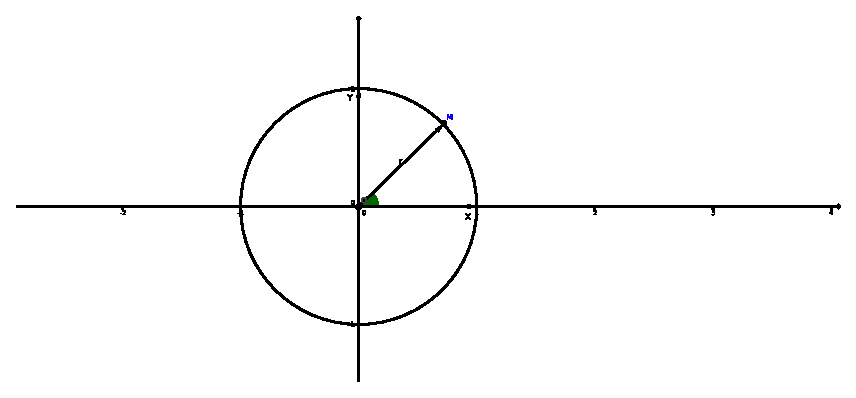
\includegraphics[scale=1, width=\textwidth]{coordpolaires.eps}
%   \caption{Représentation garphique des coordonnées polaires}
%   \label{fig:coordpol}
% \end{figure}
%
\subsection{Changements de repères}
\label{subsec:changementsderepere}
\subsubsection{Changement de repère cartésien}
\label{subsubsec:changementsdereperecart}
Soit une deuxième repère cartésiens $\Rep'=(\Omega,\vu,\vv)$ tels que dans le repère $\Rep$, $\Omega(x_1,y_1)$ $\vu(a,b)$ $\vv(c,d)$. Soit $M$ un point de $\P$ de coordonnées $(x,y)$ dans le repère $\Rep$ et $(X,Y)$ dans le repère $\Rep'$.
On a ainsi d'une part
\begin{equation}
 \vect{OM}=x \vi+ y \vj, 
\end{equation}
et d'autre part
\begin{equation}
  \vect{OM}=\vect{O\Omega}+\vect{\Omega M}=x_\Omega \vi + y_\Omega \vj + X \vu +Y\vv.
\end{equation}
Comme
\begin{equation}
  \begin{cases}
    \vu=a \vi + b \vj \\
    \vv=c\vi+d\vj
  \end{cases};
\end{equation}
alors
\begin{equation}
 \vect{OM}=(x_\Omega+aX+cY)\vi+(y_\Omega+bX+dY) \vj. 
\end{equation}
Par unicité des coordonnées on a
\begin{equation}
  \begin{cases}
    x=x_\Omega+aX+cY\\
    y=y_\Omega+bX+dY
  \end{cases}.
\end{equation}
%
\subsubsection{Formules de changement de bases orthonormales directes (BOND)}
\label{subsubsec:formuledechangementdeBOND}
On considére que $\Rep$ est un repère orthonormal direct (ROND). Soit $(\vu,\vv)$ une base orthonormale directe de $\Rep$. Pour tout réel $\theta$ on définit
\begin{align}
 \vect{u_\theta}&=\cos \theta \vi + \sin \theta \vj; \\
 \vect{v_\theta}&=\cos \theta \vj -\sin \theta \vi .
\end{align}
Il existe un réel $\varphi$ tel que $\vu=\vect{u_\varphi}$ et $\vv=\vect{v_\varphi}$.
\begin{proof}
  Soit $\varphi$ le réel tel que $\congru{\varphi}{(\vi,\vu)}{2\pi}$. Alors, $\vu$ est l'unique vecteur unitaire tel que $\congru{\varphi}{(\vi,\vu)}{2\pi}$, donc $\vu=\vect{u_\varphi}$. De plus le vecteur $\vv$ est unitaire et $(\vi,\vv)=\congru{(\vi,\vu)+(\vu,\vv)}{\varphi+\frac{\pi}{2}}{2\pi}$. Le vecteur $\vv$ est l'unique vecteur unitaire tel que $(\vi,\vv)=\varphi+\frac{\pi}{2}$ donc $\vv=\vect{v_\varphi}$.
\end{proof}
Soit un point $M$ du plan $\P$, on note $(x,y)$ ses coordonnées dans $\Rep$ et $(X,Y)$ dans $\Rep'$. Alors
\begin{equation}
  \begin{cases}
    x=\cos \varphi X - \sin \varphi Y \\
    y=\sin \varphi X + \cos \varphi Y
  \end{cases}.
\end{equation}
En inversant ce système d'équations, on obtient
\begin{equation}
  \begin{cases}
    X=\cos \varphi x + \sin \varphi y\\
    Y=-\sin \varphi x + \cos \varphi y
  \end{cases}.
\end{equation}
%
\subsubsection{Coordonnées cartésiennes et coordonnées polaires}
\label{subsubsec:coordpoletcoordcart}
On considére que $\Rep$ est un repère orthonormal direct. On considère un point $M$ de coordonnées cartésiennes $(x,y)$ et dont un s.c.p.\ est $(\rho,\theta)$ alors
\begin{equation}
 \vect{OM}=x \vi+y\vj=\rho \cos \theta \vi + \rho \sin \theta \vj.
\end{equation}
On en déduit alors par unicité des coordonnées cartésiennes que $x=\rho \cos \theta$ et $y=\rho \sin \theta$. Donc si on sait que $\rho$ est strictement positif alors $\rho=\sqrt{x^2+y^2}$.
%
\subsection{Équations cartésiennes et polaires}
\label{subsec:equationspoletcoordcart}
Soit $X$ une partie du plan $\P$ munie du repère $\Rep$.
\begin{defdef}
  \begin{enumerate}
  \item Soit $F:\R^2 \longmapsto \R$ une application, on dit que $F(x,y)=0$ est une équation cartésienne de $X$ dans $\Rep$ si et seulement si pour tout point $M$ du plan on a
    \begin{equation}
      M \in X \iff \exists (x,y)\in\R^2 \quad F(x,y)=0.
    \end{equation}
  \item Soit $G:\R^2 \longmapsto \R$ une autre application, on dit que $G(r,\theta)=0$ est une équation polaire de $X$ dans $\Rep$ si et seulement si pour tout point $M$ du plan on a
      \begin{equation}
        M \in X \iff \exists (\rho, \theta)\in\R^2 \quad G(\rho,\theta)=0.
      \end{equation}
  \item Soit $I$ un intervalle réel et $\fonction{f}{I}{\R^2}{t}{(x(t),y(t))}$. On dit que $f$ est un paramétrage de la partie $X$ du plan dans le repère $\Rep$ si et seulement si $X=\enstq{M(x(t),y(t))}{t \in I}$.
  \end{enumerate}
\end{defdef}
%
\subsubsection{Applications}
\label{subsubsec:applicationeqcartetpol}
\paragraph{Équation d'un cercle}
\label{par:eqcercle}
Soit $\Omega \in \P \setminus\{O\}$ et $(R,\varphi)$ un s.c.p.\ de $\Omega$ avec $R>0$. L'ensemble $\courbe$ est le cercle de centre $\Omega$ passant par $O$. Il s'agit de donner une équation polaire de ce cercle.
\begin{proof}[Analyse]
Soit $M$ un point du cercle et soit $(\rho, \theta)$ un s.c.p.\ de $M$. 

Dans un premier temps, on commence par supposer que $\rho >0$. Le triangle $O\Omega M$ est isocèle en $\Omega$. Soit $H$ le projeté orthogonal de $\Omega$ sur $(OM)$ alors $H$ est le milieu de $[OM]$ et
\begin{equation}
 \cos(\theta - \varphi)=\frac{OH}{OM}=\frac{\rho/2}{R}, 
\end{equation}
donc
\begin{equation}  
  \rho=2R \cos(\theta-\varphi). 
\end{equation}

Dans un deuxième temps, on suppose que $\rho$ est nul, alors $M=O$. Tout couple $(0,\theta)$ est un s.c.p.\ de $M$ et en particulier $(0,\varphi+\frac{\pi}{2})$ et donc $2R \cos(\varphi+\frac{\pi}{2} - \varphi)=0=\rho$. 

Dans un troisième et dernier temps, on suppose que $\rho <0$, alors $(-\rho, \theta+\pi)$ est un autre s.c.p.\ de $M$. Donc
\begin{equation}
  -\rho = 2R \cos(\theta+\pi-\varphi),
\end{equation}
soit en simplifiant
\begin{equation}
  \rho=2R\cos(\theta-\varphi).
\end{equation}

On a donc montré que pour tous point $M$ du cercle, il existe un s.c.p.\ $(\rho,\theta)$ de $M$ tel que $\rho=2R\cos(\theta-\varphi)$.
\end{proof}
\begin{proof}[Synthèse]
Soit un point $M$ du plan admettant un s.c.p.\ $(\rho,\theta)$ tel que $\rho=2R\cos(\theta-\varphi)$. Si on se place dans le repère $\Rep' (O,\vect{u_\varphi}, \vect{v_\varphi})$ alors $\Omega =(R,0)$ dans $\Rep'$. Un s.c.p.\ de $M$ dans $\Rep'$ peut aussi être $(\rho,\theta-\varphi)$. Alors, dans $\Rep'$, on a $M=(\rho \cos(\theta-\varphi), \rho \sin(\theta-\varphi))$. Ainsi~:
\begin{align}
  {\Omega M}^2&=(\rho\cos(\theta-\varphi)-R)^2 + (\rho\sin(\theta-\varphi))^2 \\
  &= \rho^2 \cos^2(\theta-\varphi)+R^2 - 2R\cos(\theta-\varphi)\rho + \rho^2 \sin^2(\theta-\varphi) \\
  &= \rho^2 + R^2 - \rho^2\\
  &= R^2.
\end{align}
On a montré que si $M$ admettait un s.c.p.\ vérifiant l'équation, alors il est sur le cercle.
\end{proof}
%
\paragraph{Équation d'une droite}
\label{par:eqdroite}
Soit $H \in \P\setminus\{O\}$ dont un s.c.p.\ est $(R,\varphi)$ avec $R>0$. Soit $\Dr$ la droite passant par $H$ et orthogonale à $(OH)$. Il s'agit de donner une équation polaire de $\Dr$.
\begin{proof}[Analyse]
  Soit $M$ un point de $\Dr$ et $(\rho,\theta)$ un s.c.p.\ de $M$. puisque $O \notin \Dr$ alors $\rho \neq 0$. Commençons en supposant que $\rho>0$ alors
  \begin{equation}
    \cos(\theta-\varphi)=\frac{OH}{OM}=\frac{R}{\rho},
  \end{equation}
  et donc $R=\rho \cos(\theta-\varphi)$. 

  Si $\rho<0$ alors $(-\rho,\theta+\pi)$ est un autre s.c.p.\ de $M$ et on a encore $\rho\cos(\theta-\varphi)=R$. On a donc montré que tout point de $\Dr$ admet un s.c.p.\ $(\rho, \theta)$ tel que $\rho\cos(\theta-\varphi)=R$.
\end{proof}
\begin{proof}[Synthèse]
Soit $M$ un point qui admet un s.c.p.\ $(\rho,\theta)$ vérifiant l'équation
\begin{equation}
  \rho\cos(\theta-\varphi)=R.
\end{equation}
On se place dans le repère $(O,\vect{u_\varphi}, \vect{v_\varphi})$. Alors $H$ est de coordonnées $(R,O)$ et $M$ est de coordonnées $(\rho\cos(\theta-\varphi), \rho\sin(\theta-\varphi))$~\footnote{parce que $(\rho, \theta-\varphi)$ est un s.c.p.\ de $M$}. Du coup le vecteur $\vect{HM}$ est de coordonnées $(0, \rho\sin(\theta-\varphi))$ et on a $\vect{u_\varphi}$ de coordonnée $(1,0)$. 

On voit donc que ces deux vecteurs sont orthogonaux et donc que $M$ est sur la droite $\Dr$.
\end{proof}

\section{Produit scalaire}
\label{sec:prodscalaire}
\subsection{Définition géométrique}
\begin{defdef}
  Soient $\vu$ et $\vv$ deux vecteurs du plan. On définit le réel $\vu \cdot \vv$ appelé produit scalaire de $\vu$ et $\vv$ 
  \begin{itemize}
  \item si $\vu$ est nul ou si $\vv$ est nul par $\vu \cdot \vv=0$;
  \item si $\vu$ est non nul et si $\vv$ est non nul par $\vu \cdot \vv=\norme{\vu}\norme{\vv}\cos(\vu, \vv)$.
  \end{itemize}
\end{defdef}
\begin{prop}
   Soient deux vecteurs $\vu$ et $\vv$, ils sont orthogonaux si et seulement si leur produit scalaire est nul.
\end{prop}
\begin{proof}
Les vecteurs $\vu$ et $\vv$ sont orthogonaux si et seulement si l'un des deux est nul ou s'il forment un angle droit. C'est à dire si et seulement si l'un des deux est nul ou si le cosinus de leur angle est nul donc si et seulement si leur produit scalaire est nul d'après la définition.
\end{proof}

Supposons maintenant que $\vu$ soit non nul, alors on définit un vecteur unitaire $\vect{a}=\frac{\vu}{\norme{\vu}}$. Soit le vecteur $\vect{b}$ unitaire et unique tel que $(\vect{a},\vect{b})=\frac{\pi}{2}$. Le couple $(\vect{a},\vect{b})$ forme donc une base orthonormale directe. Dans cette base, le vecteur $\vu$ a pour coordonnées $(\norme{\vu},0)$ et si $\vv$ est non nul alors il existe un s.c.p.\ dans le repère $(\vect{a},\vect{b})$, c'est $(\norme{\vv}, (\vu,\vv))$. Les coordonnées cartésiennes de $\vv$ dans le repère $(\vect{a},\vect{b})$ sont $(\norme{\vv}\cos(\vu,\vv),\norme{\vv}\sin(\vu,\vv))$. Alors $\vu \cdot \vv=X_{\vu}X_{\vv}$ (si $\vv$ est nul alors l'expression est encore vraie). On note $\Dr$ la droite passant par $O$ dirigée par $\vu$. Soient $M$ tel que $\vect{OM}=\vu$, $N$ tel que $\vect{ON}=\vv$ et $H$ le projeté orthogonal de $N$ sur $\Dr$. Alors $\vu \cdot \vv=\vect{OM} \cdot \vect{ON}= \overline{OM}~\overline{OH}$.

\subsection{Propriétés algébriques}
\begin{prop}
  Le produit scalaire est une forme bilinéaire et symétrique, c'est à dire que pour trois vecteur $\vu, \vv, \vw$ quelconques du plan et un réel $\lambda$ on a~:
  \begin{gather}
    \vu \cdot \vv = \vv \cdot \vu;\\
    \vu \cdot (\lambda \vv) = \lambda (\vu\cdot \vv) \qquad \vu \cdot (\vv + \vw)=\vu \cdot \vv + \vu \cdot \vw;\\
    (\lambda \vu) \cdot \lambda \vv = \lambda (\vu \cdot \vv) \qquad (\vv + \vw) \vu=\vv \cdot \vu + \vw \cdot \vv;\\
    \vu \cdot \vu = \norme{\vu}^2.
  \end{gather}
\end{prop}
\begin{proof}
  Si $\vu$ ou $\vv$ est nul alors leur produit scalaire est nul, donc il commute. Sinon puisque la fonction cosinus est paire et puisque $(\vu,\vv)=-(\vv,\vu)$ alors la proposition est vraie.

  Si $\vu$ est nul alors l'égalité est vraie et sinon on se place dans la base $(\vect{a},\vect{b})$ définie précédemment et on a 
  \begin{equation}
    \vu \cdot (\lambda \vv) = X_{\vu} X_{\lambda \vv}=\lambda X_{\vu} X_{\vv}=\lambda \vu \cdot \vv,
  \end{equation}
  et on démontre de la même manière la distributivité à droite. La linéarité à gauche découle de la symétrie et de la linéarité à droite du produit scalaire.
   
  Si le vecteur $\vu$ est nul alors l'égalité est vraie, sinon puisque $(\vu,\vu)=0$ alors on a l'égalité.  
\end{proof}
\begin{prop}
  Soient $(\vi,\vj)$ une BON, deux vecteurs $\vu$ et $\vv$ de coordonnées cartésiennes $(x,y)$ et $(x',y')$ dans $(\vi,\vj)$. Alors $\vu \cdot \vv=xx+yy'$
\end{prop}
\begin{proof}
  On peut décomposer le produit scalaire sur la base orthonormale du plan $(\vi,\vj)$~:
  \begin{align}
    \vu \cdot \vv &= (x \vi + y \vj) \cdot (x' \vi + y' \vj) \\
    &= x x' \vi \cdot \vi + xy' \vi \cdot \vj + yx' \vi \cdot \vj + yy' \vj \cdot \vj\\
    & = xx' +yy'.
  \end{align}
  Puisque les vecteurs $\vi$ et $\vj$ sont unitaires et orthogonaux.
\end{proof}
\begin{prop}
  Soient $(\vi,\vj)$ une BON, deux vecteurs $\vu$ et $\vv$ des vecteurs d'affixes respectives $z$ et $z'$ dans la BON\@. Alors $\vu \cdot \vv=\Re(\bar{z} z')$.
\end{prop}
\begin{proof}
  On note $z=x+\ii y$ et $z'=x'+\ii y'$ avec $(x,y)$ les coordonnées cartésiennes de $\vu$ et $(x',y')$ les coordonnées cartésiennes de $\vv$. Alors
  \begin{equation}
    \bar{z} z' = (x-\ii y)(x'+\ii y')=xx'+yy' + \ii(xy'-x'y).
  \end{equation}
  Alors $\vu \cdot \vv=xx' + yy'=\Re(\bar{z} z')$.
\end{proof}
\begin{prop}[Théorème d'Al-Kashi]
  Dans un triangle ABC quelconque, on a 
  \begin{equation}
    BC^2=AC^2+AB^2-2 AB \times AC \cos(\widehat{BAC}).
  \end{equation}
\end{prop}
\begin{proof}
  \begin{align}
    BC^2=\vect{BC} \cdot \vect{BC}& =(\vect{BA}+\vect{AC})^2 \\
    & = BA^2+AC^2 +2 \vect{BA} \cdot \vect{AC} \\ 
    & = BA^2+AC^2 -2 \vect{AB} \cdot \vect{AC}\\ 
    & = BA^2+AC^2 -2 AB \times AC \cos(\widehat{BAC}).
  \end{align}
\end{proof}

\subsection{Lignes de niveaux du produit scalaire}
Soient $A$ un point du plan fixe et $\vu$ un vecteur fixe, on considère
\begin{equation}
  \fonction{\psi}{\P}{\R}{M}{\vu\cdot\vect{AM}}.
\end{equation}
Il s'agit de déterminer les ensembles
\begin{equation}
  \forall \lambda \in \R \quad  X_\lambda = \enstq{M \in \P}{\psi(M)=\lambda}=\enstq{M \in \P}{\vu \cdot \vect{AM} = \lambda}.
\end{equation}
\begin{itemize}
\item[Cas 1] si $\vu$ est nul alors pour tous point $M$ du plan on a $\psi(M)=0$. Ainsi si $\lambda=0$ alors $X_0=\P$ et sinon alors $X_\lambda=\emptyset$;
\item[Cas 2] si $\vu$ est non nul alors on commence par chercher les éventuels éléments $M$ de $X_\lambda$ tels que $\vect{AM}$ soit colinéaire à $\vu$, c'est à dire si et seulement s'il existe un réel $\alpha$ tel que $\vect{AM}=\alpha \vu$. On a donc la suite d'équivalence :
  \begin{align}
    M \in X_\lambda &\iff  \vu \cdot \vect{AM}=\lambda \\
    & \iff \alpha \norme{\vu}^2=\lambda \\
    & \iff \alpha= \frac{\lambda}{\norme{\vu}^2}.
  \end{align}
  Soit donc le point $H_\lambda$ défini par $\vect{AH_\lambda}=\frac{\lambda}{\norme{\vu}^2} \vu$ ($H_\lambda \in X_\lambda$). Alors pour un point $M$ quelconque, on a
  \begin{align}
    M \in X_\lambda &\iff  \vu \cdot \vect{AM}=\lambda \\
    &\iff  \vu \cdot \vect{AM} = \vu \cdot \vect{AH_\lambda} \\
    &\iff  \vu \cdot \vect{H_\lambda M}=0.
  \end{align}
  Ce qui est équivalent à $\vect{H_\lambda M}$ et $\vu$ orthogonaux. On en déduit que $X_\lambda$ est la droite passant par $H_\lambda$ orthogonale à $\vu$.
\end{itemize}

\emph{Conséquences}~:
\begin{enumerate}
\item Si $\lambda = 0$ alors $X_0$ est la droite passant par $A$ et orthogonale à $\vu$. Si $\Dr$ est une droite, si on connaît un point $A(a,b)$ de $\Dr$ et un vecteur normal $\vect{n}(\alpha,\beta)$, on peut facilement déduire une équation cartésienne de $\Dr$. Soit un point $M(x,y)$ du plan, alors~:
  \begin{align}
    M \in \Dr  \iff & \vect{n} \cdot \vect{AM}=0 \\
    \iff & \alpha(x-a)+\beta(y-b)=0\\
    \iff & \alpha x + \beta y=a \alpha + b \beta;
  \end{align}
\item Soient $A=O$, $\Dr$ une droite quelconque du plan, H le projeté orthogonal de O sur $\Dr$, $\vu$ un vecteur normal unitaire de $\Dr$. Il existe un réel $\varphi$ tel que $\vu=\vect{u_\varphi}$ et on note $\rho=\vu \cdot \vect{OH}$ alors pour tous point $M(x,y)$ on a 
  \begin{align}
    M \in \Dr & \iff \vect{MH} \cdot \vect{OM}=0 \\
    & \iff \vect{MH} \cdot \vu =0 \\
    & \iff \vect{MO} \cdot \vu +\vect{OH} \cdot \vu=0\\
    & \iff \vu \cdot \vect{OM}=\rho\\
    & \iff x \cos \varphi + y \sin \varphi=\rho.
  \end{align}
  C'est l'équation normale de la droite $\Dr$.
\end{enumerate}

\section{Déterminant}
\subsection{Définition géométrique}
\begin{defdef}
  Soient $\vu$ et $\vv$ deux vecteurs. On définit le réel $\Det(\vu;\vv)$ appelé déterminant de $\vu$ et $\vv$ par:
  \begin{itemize}
  \item si $\vu$ ou $\vv$ est nul alors $\Det(\vu;\vv)=0$;
  \item sinon $\Det(\vu;\vv)=\norme{\vu}\norme{\vv} \sin(\vu,\vv)$.
  \end{itemize}
\end{defdef}
\begin{prop}
  Deux vecteurs du plan sont colinéaires si et seulement si leur déterminant est nul. Deux vecteurs forment une base (in)directe si leur déterminant est positif (négatif).
\end{prop}
\begin{proof}
  Soient $\vu$ et $\vv$ deux vecteurs du plan. Alors $\vu$ et $\vv$ sont colinéaires si et seulement si l'un des deux est nul ou $\congru{(\vu,\vv)}{0}{\pi}$. C'est-à-dire si et seulement si l'un des deux est nul ou $ \sin(\vu,\vv) = 0$, c'est à dire si et seulement si leur déterminant est nul.

  Supposons que $(\vu,\vv)$ soit non congru à 0 modulo $\pi$ alors on considère $\theta$ la mesure principale de l'angle $(\vu,\vv)$, $\theta \in \intervalleof{-\pi}{\pi}$. Si le déterminant est positif, alors $\sin \theta$ est positif donc dans $\intervalleof{-\pi}{\pi }$, $\theta$ est positif. C'est donc un base directe. Avec un raisonnement équivalent on montre que si le déterminant est négatif alors la base est indirecte.
\end{proof}

Si $\vu$ est non nul alors on introduit la base $(\vect{a},\vect{b})$ (vue à la section~\ref{sec:prodscalaire}). On avait vu que dans cette base, les coordonnées de $\vu$ et $\vv$ étaient $\vu(\norme{\vu},0)$ et $\vv(\norme{\vv} \cos(\vu,\vv),\norme{\vv} \sin(\vu,\vv))$. Donc $\Det(\vu;\vv)=X_{\vu} Y_{\vv}$. De façon géométrique le déterminant de $\vu$ et $\vv$ représente l'aire du parallélogramme basé sur ces deux vecteurs.

\subsection{Propriétés algébriques}
\begin{prop}
Pour $\vu, \vv, \vw$ trois vecteurs et $\lambda$ un réel on a~:
\begin{gather}
  \Det(\vu,\vu)=0;\\
  \Det(\vu, \vv)=-\Det(\vv, \vu);\\
  \Det( \lambda \vu, \vv) = \lambda \Det(\vu, \vv) \quad \Det(\vu+ \vv, \vw) =\Det(\vu, \vv) + \Det(\vv, \vw);\\
  \Det(\vu, \lambda \vv) = \lambda \Det(\vu, \vv) \quad \Det(\vu, \vw + \vv) =\Det(\vu, \vw) + \Det(\vu, \vv)
\end{gather}
\end{prop}
\begin{proof}
\begin{enumerate}
\item On a déjà vu que si les vecteurs sont colinéaires alors le déterminant est nul.
\item Si l'un des deux vecteur est nul alors puisque leur déterminant est nul, la formule est vraie. Sinon puisque la fonction sinus est impaire, alors le résultat est vrai aussi.
\item Si l'un des deux vecteur est nul alors puisque leur déterminant est nul, la formule est vraie. Sinon on se place dans la base $(a,b)$ définie dans la section~\ref{sec:prodscalaire} et dans ce cas $\Det( \lambda \vu, \vv) = X_{\vu} Y_{\lambda \vv}=\lambda X_{\vu} Y_{\vv}=\lambda \Det(\vu, \vv)$ et aussi pour l'additivité : $\Det(\vu, \vw + \vv)=X_{\vu} Y_{\vv + \vw}= X_{\vu} Y_{\vv} + X_{\vu} Y_{\vw}=\Det(\vu, \vw) + \Det(\vu, \vv)$
\item La dernière formule se déduit des deux précédentes propriétés.
\end{enumerate}
\end{proof}
\begin{prop}
Soient $(\vi,\vj)$ une BOND, $\vu$ et $\vv$ deux vecteurs de coordonnées cartésiennes respectives $(x,y)$ et $(x',y')$ dans $(\vi,\vj)$. Alors 
\begin{equation}
  \Det(\vu,\vv)=xy'-yx'=\begin{vmatrix} x&x'\\y&y'\end{vmatrix}.
\end{equation}
\end{prop}
\begin{proof}
  Puisque le déterminant est bilinéaire, on peut écrire que
  \begin{equation}
    \Det(\vu,\vv)=xx' \Det(\vi,\vi) + xy' \Det(\vi,\vj)+x'y\Det(\vj,\vi)+yy'\Det(\vj,\vj).
  \end{equation}
  Puisque $(\vi,\vj)$ est une BOND, on a le résultat.
\end{proof}
\begin{prop}
  Soient $(\vi,\vj)$ une BOND, $\vu$ et $\vv$ deux vecteurs d'affixe respectives $z$ et $z'$, alors 
\begin{equation}
  \Det(\vu,\vv)=\Im(\bar{z}z').
\end{equation}
\end{prop}
\begin{proof}
  Voir la preuve de la proposition correspondante au produit scalaire.
\end{proof}
\begin{prop}
  Pour tous vecteurs $\vu$ et $\vv$~:
  \begin{equation}
    (\vu \cdot \vv)^2+\Det(\vu,\vv)^2=\norme{\vu}^2 \norme{\vv}^2.
  \end{equation}
\end{prop}
\begin{proof}
  Si l'un des deux vecteur est nul la formule est vérifiée par $0+0=0$. Sinon le résultat découle de l'égalité $\sin^2+\cos^2=1$.
\end{proof}

\subsection{Lignes de niveaux du déterminant}
Soient $A$ un point fixe du plan, $\vu$ un vecteur fixe, $\lambda$ un réel fixe. On cherche à déterminer
\begin{equation} 
  Y_\lambda = \enstq{M \in \P}{\Det(\vu, \vect{AM})=\lambda}.
\end{equation}
\begin{enumerate}
\item[Cas 1] Si le vecteur $\vu$ est nul alors si $\lambda$ est nul $Y_0=\P$ et si $\lambda$ n'est pas nul alors $Y_\lambda=\emptyset$.
\item[Cas 2] Si le vecteur $\vu$ est non nul, alors on considère le vecteur $\vv$ tel que $\norme{\vv}=\norme{\vu}$ et $\congru{(\vu,\vv)}{\frac{\pi}{2}}{2\pi}$. On commence par chercher un point $M$ de $Y_\lambda$ qui vérifie $\vect{AM}$ colinéaire à $\vv$~:
  \begin{align}
    \begin{cases} \exists \alpha \in \R \quad \vect{AM}=\alpha \vv \\  M \in Y_\lambda\end{cases}  \iff & \begin{cases}\exists \alpha \in \R \quad \vect{AM}=\alpha \vv \\ \Det(\vu,\vect{AM})=\lambda\end{cases} \\
    \iff & \begin{cases} \exists \alpha \in \R \quad \vect{AM}=\alpha \vv \\ \lambda=\alpha \norme{\vu}^2\end{cases} \\
    \iff & \vect{AM}=\frac{\lambda}{\norme{\vu}^2} \vv.
  \end{align}
  Soit donc $H_\lambda$ le point tel que $\vect{AH_\lambda}=\frac{\lambda}{\norme{\vu}^2} \vv$. Pour tout point $M$ du plan, on a
  \begin{align}
    M \in Y_\lambda \iff & \Det(\vu,\vect{AM})=\lambda \\ 
    \iff & \Det(\vu,\vect{AM})=\Det(\vu,\vect{AH_\lambda}) \\ 
    \iff & \Det(\vu,\vect{H_\lambda M})=0
  \end{align}
  Donc $Y_\lambda$ est la droite passant par $H_\lambda$ et dirigée par $\vu$.
\end{enumerate}

\emph{Remarques}~:
\begin{enumerate}
\item Le vecteur $\vv$ est défini par la propriété suivante~: pour tout vecteur $\vw$, on a $\vv \cdot \vw=\Det(\vu,\vw)$.
  \begin{proof}
    Si le vecteur $\vw$ est nul alors comme le produit scalaire est nul et le déterminant aussi, c'est bon. Sinon alors 
    \begin{align}
      \vv\cdot\vw&=\norme{\vv}\norme{\vw}\cos(\vv,\vw)\\ 
      &=\norme{\vu}\norme{\vw} \cos((\vv,\vu) + (\vu,\vw))\\ 
      &=\norme{\vu}\norme{\vw} \cos\left(\vu,\vw -\frac{\pi}{2} \right)\\ 
      &=\norme{\vu} \norme{\vw} \sin(\vu,\vw) \\ 
      &=\Det(\vu,\vw).
    \end{align}
  \end{proof}
  Le vecteur $\vv$ est l'unique vecteur à vérifier cette propriété : Supposons qu'un deuxième vecteur $\vv'$ vérifie la propriété, alors pour tout vecteur $\vw$ on a $\vv \cdot \vw =\vv' \cdot \vw$ alors $(\vv-\vv') \cdot \vw=0$ et en particulier si $\vw=\vv-\vv'$ alors $\norme{\vv-\vv'}^2=0$ alors $\vv=\vv'$.
\item La méthode précédente permet d'obtenir une équation pour les droites $\Dr$ dont on connaît :
  \begin{itemize}
  \item un point $A$ de $\Dr$ et un vecteur directeur de $\Dr$
    \begin{equation}
      \forall M \in \P \quad M \in \Dr \iff \Det(\vu, \vect{AM})=0,
    \end{equation}
  \item deux points $A$ et $B$ de $\Dr$ 
    \begin{equation}
      \forall M \in \P \quad M \in \Dr \iff \Det(\vect{AB}, \vect{AM})=0.
    \end{equation}
  \end{itemize}
\end{enumerate}

\section{Droites}
\index{sec:droites}
\subsection{Équations de droites}

On se place dans un repère orthonormal $(O,\vi,\vj)$.
\begin{prop}
Trois points $A(a_1,b_1)$ $B(a_2,b_2)$ et $C(a_3,b_3)$ du plan sont alignés si et seulement si
\begin{equation}
  \Det(\vect{AB},\vect{AC})=
  \begin{vmatrix}
    a2-a1&a3-a2\\
    b2-b1&b3-b1
  \end{vmatrix} =0.
\end{equation}
\end{prop}
\begin{prop}
On considère une droite $\Dr$ passant par $A(a_1,b_1)$ et dirigé par $\vu(a,b)$. L'équation paramétrique de $\Dr$ est
\begin{equation}
 \forall \lambda \in \R \begin{cases} x=a_1+\lambda a \\ y=b_1+ \lambda b\end{cases}. 
\end{equation}
L'équation cartésienne de $\Dr$ est donnée par la condition sur le déterminant. Si un point $M$ du plan est sur la droite alors $\Det(\vu,\vect{AM})=0$ qui est équivalent à l'équation $a(y-b_1)-b(x-a_1)=0$.
\end{prop}
Si la droite $\Dr$ a pour équation cartésienne
\begin{equation}
 ax+by+c=0 \quad ((a,b) \neq (0,0)),
\end{equation}
alors un vecteur directeur de $\Dr$ est $\vu(-b,a)$.
\begin{prop}
  On considère une droite $\Dr$ passant par $A(a_1,b_1)$ et $B(a_2,b_2)$ avec $A \neq B$. L'équation paramétrique de $(AB)$ est
  \begin{equation}
    \forall \lambda \in \R \begin{cases} x=a_1+\lambda (a_2-a_1) \\ y=b_1+ \lambda (b_2-b_1)\end{cases}.
  \end{equation}
L'équation cartésienne de $\Dr$ est donnée par la condition sur le déterminant. Si un point $M$ du plan est sur la droite $(AB)$ alors $\Det(\vect{AB},\vect{AM})=0$ qui est équivalent à l'équation $(a_2-a_1)(y-b_1)-(b_2-b_1)(x-a_1)=0$.
\end{prop}
\begin{prop}
  Soient un point $A(a_1,b_1)$ et un vecteur $\vv(v_1,v_2)$. On considère la droite $\Dr$ passant par $A$ et dont $\vv$ est un vecteur normal. Alors pour tous point $M(x,y)$ du plan, $M$ est sur la droite si et seulement si $\vect{AM}\cdot\vv=0$, c'est-à-dire si et seulement si $v_1(x-a_1)+v_2(y-b_1)=0$.
\end{prop}
Si $\Dr$ admet pour équation cartésienne $ax+by+c=0$ avec $(a,b) \neq (0,0)$, alors un vecteur normal de $\Dr$ est $\vn(a,b)$.
\begin{prop}
  Soit $\Dr$ une droite et $\vn=\vect{v_\varphi}$ un vecteur normal unitaire de $\Dr$. Soit $H$ le projeté orthogonal de $O$ sur $\Dr$.
  \begin{equation}
    M(x,y) \in \Dr \iff x\cos\phi + u \sin\phi=p.
  \end{equation}
\end{prop}

\subsection{Distance d'un point à une droite}

Soient $\Dr$ une droite et $A$ un point. On cherche à déterminer la plus courte distance de $A$ a un point de la droite et à montrer qu'elle est atteinte en un seul point. Soit $H$ le projeté orthogonal de $A$ sur la droite $\Dr$. Pour tout point $M$ du plan, on peut appliquer le théorème de Pythagore sur le triangle rectangle $AHM$ : $AM^2=AH^2+HM^2 \geq AH^2$. Donc $AM \geq AH$ et on a $AM=AH \iff H=M$. Ainsi $d(A,\Dr)=AH$ et elle n'est atteinte qu'en un seul point : le projeté orthogonal de $A$ sur la droite $\Dr$.% On représente le problème par la figure \ref{fig:dist}
% \begin{figure}[!h]
%   \centering
%   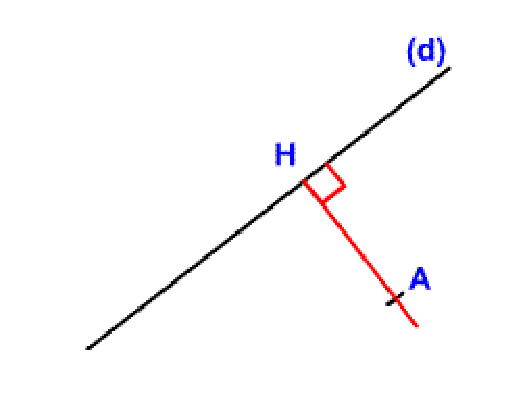
\includegraphics[scale=0.5]{distance-point-droite.eps}
%   \caption{Distance d'un point à une droite}
%   \label{fig:dist}
% \end{figure}

\emph{Expressions de $d(A,\Dr)$}~:
On montre ici plusieurs cas de figure selon la situation~:
\begin{enumerate}
\item Soit un vecteur unitaire $\vu$ normal à $\Dr$ et $M$ un point de $\Dr$ quelconque. Alors
  \begin{equation}
    \vu \cdot \vect{AM} = \vu \cdot \vect{AH} + \vu \cdot \vect{HM}=\vu \cdot \vect{AH},
  \end{equation}
  puisque $\vu$ et $\vect{AH}$ sont colinéaires, on peut écrire que~:
  \begin{equation}
    \forall M \in \Dr \quad d(A,\Dr)=|\vu \cdot \vect{AH}|
  \end{equation}
\item Soit un vecteur $\vu=\vu_\varphi(\cos \varphi, \sin \varphi)$ et si $\Dr$ admet pour équation normale
  \begin{equation}
    x \cos \varphi + y \sin \varphi=p,
  \end{equation}
  avec $A(a_1,b_1)$, alors pour tout point $M(x,y)$ de la droite $\Dr$ on a
  \begin{align}
    \vu \cdot \vect{AM} &= \cos \varphi (x-a_1) + \sin \varphi (y-b_1)\\
    &= p-a_1\cos\varphi -b_1\sin\varphi.
  \end{align}
  Ainsi
  \begin{equation}
    d(A,\Dr)=|p-a_1\cos\varphi-b_1\cos\varphi|.
  \end{equation}
\item Si $\Dr$ a pour équation polaire $\rho\cos(\theta-\varphi)=p$ alors $x \cos \varphi + y \sin \varphi=p$ est une équation normale de $\Dr$. Soit $(\rho_A,\theta_A)$ un s.c.p.\ de A, alors $a_1=\rho_A\cos\theta_A \ b_1=\rho_A\sin\theta_A$, donc
  \begin{equation}
    d(A,\Dr)=|p-\rho_A\cos(\theta_A-\varphi)|.
  \end{equation}
\item Si $\Dr$ admet pour équation cartésienne $ax+by+c=0$ avec $(a,b) \neq (0,0)$, soient $A(x_0,y_0)$ et $\vu \left(\frac{a}{\sqrt{a^2+b^2}}, \frac{b}{\sqrt{a^2+b^2}}\right)$ un vecteur normal unitaire de $\Dr$. Alors pour tout point $M(x,y)$ de la droite $\Dr$ on a
  \begin{equation}
      \vu\cdot\vect{AM}=\frac{a(x-x_0)+b(y-y_0)}{\sqrt{a^2+b^2}}=\frac{-c-ax_0-by_0}{\sqrt{a^2+b^2}}.
    \end{equation}
    Donc
    \begin{equation}
      d(A,\Dr)=\frac{c+ax_0+by_0}{\sqrt{a^2+b^2}}.
    \end{equation}
  \end{enumerate}
  
\subsection{Positions relatives de droites}
 On dit que deux droites du plan sont parallèles si elles admettent des vecteurs directeurs colinéaires et on dit qu'elles sont orthogonales si elles admettent des vecteurs directeurs orthogonaux.

 \begin{prop}
Soient deux droites du plan $\Dr_1$ et $\Dr_2$ deux droites d'équations cartésiennes respectives~:
\begin{align}
  a_1x+b_1y+c_1&=0 \quad (a_1,b_1)\neq(0,0)\\
  a_2x+b_2y+c_2&=0 \quad (a_2,b_2)\neq(0,0).
\end{align}
\begin{enumerate}
\item $\Dr_1$ et $\Dr_2$ sont parallèles si seulement si $(a_1,b_1)$ et $(a_2,b_2)$ sont proportionnels. Ce qui équivaut encore à $
  \begin{vmatrix}
    a_1 & a_2 \\
    b_1 & b_2
  \end{vmatrix}=0$.
Elle sont alors disjointes ou confondues.
\item Sinon elles se coupent en un unique point.
\end{enumerate}
 \end{prop}
 \begin{proof}
   \begin{enumerate}
   \item $\vect{m}_1(a_1,b_1)$ et $\vect{m}_2(a_2,b_2)$ sont des vecteurs normaux de $\Dr_1$ et $\Dr_2$. $\Dr_1$ et $\Dr_2$ sont parallèles équivaut à $\vect{m}_1(a_1,b_1)$ et $\vect{m}_2(a_2,b_2)$ sont colinéaires. S'il existe $I \in \Dr_1 \cap \Dr_2$, $\Dr_1$ et $\Dr_2$ sont toutes les deux égales à la droite passant par $I$ de vecteur directeur $(-b_1 a_1)$, car $(-b_1 a_1)$ et $(-b_2 a_2)$ sont alors colinéaires.
     \item Sinon $
  \begin{vmatrix}
    a_1 & a_2 \\
    b_1 & b_2
  \end{vmatrix} \neq 0$ et la détermination de $\Dr_1 \cap \Dr_2$ se ramène à la résolution du système linéaire
\begin{equation}
 \begin{cases} 
   a_1x+b_1y+c_1 &=0 \\ 
   a_2x+b_2y+c_2 &=0
 \end{cases}
\end{equation}
dont le déterminant est non nul, la solution est donc unique.
   \end{enumerate}
\end{proof}
\begin{prop}
  Soient $\Dr_1$ et $\Dr_2$ deux droites d'équations cartésiennes respectives $a_1x+b_1y+c_1=0$ et $a_2x+b_2y+c_2=0$ avec $(a_1,b_1) \neq (0,0)$ et $(a_2,b_2) \neq (0,0)$. Alors elles sont orthogonales si et seulement si $a_1 a_2 + b_1 b_2=0$
\end{prop}
\begin{proof}
  Ces deux droites sont orthogonales si et seulement si leurs vecteurs directeurs $\begin{pmatrix} -b_1 \\ a_1 \end{pmatrix}$ et $\begin{pmatrix} -b_2 \\ a_2 \end{pmatrix}$ sont orthogonaux soit si et seulement si leur produit scalaire est nul, ie. $b_1 b_2 + a_1 a_2=0$
\end{proof}

\emph{Angles de droites}~:
Soient $\Dr_1$ et $\Dr_2$ deux droite, $\vu_1$ un vecteur directeur de $\Dr_1$ et $\vu_2$ un vecteur directeur de $\Dr_1$. On appelle mesure de l'angle orienté de ces deux droites tout réel $\theta$ tel que $(\vect{u_1};\vect{u_2})=\theta$.

\section{Cercles}
\label{sec:cercle}
\subsection{Caractérisation de l'appartenance à un cercle}
\label{sec:caractcercle}
On se place dans un ROND $(O,\vi,\vj)$. Soient $A(a,b)$ et $R \in \Rplusetoile$. Le cercle de centre $A$ et de rayon $R$, noté $\cercle{A}{R}$, est l'ensemble des points $M(x,y)$ tel que $AM=R$. Si un point $M(x,y)$ est sur le cercle $\cercle{A}{R}$, c'est équivalent à
\begin{align}
  AM^2=R^2 & \iff (x-a)^2+(y-b)^2=R^2\\
&\iff x^2+y^2-2ax-2by=R^2-a^2-b^2.
\end{align}
Réciproquement, Soit $X$ la partie du plan d'équation cartésienne $x^2+y^2-2ax-2by=c$ où $a$, $b$ et $c$ sont des réels, alors $(x-a)^2+(y-b)^2=c+a^2+b^2$. Trois cas de figures se présentent :
\begin{itemize}
\item si $c+a^2+b^2<0$ alors $X=\emptyset$;
\item si $c+a^2+b^2=0$ alors $x=a$, $y=b$ et donc $X=\{A\}$;
\item si $c+a^2+b^2>0$ alors soit $R=\sqrt{a^2+b^2+c}$ et $A=(a,b)$ et donc $X=\cercle{A}{R}$.
\end{itemize}
\begin{prop}
  \label{prop:cocy}
  Soit $\mathcal{C}$ un cercle de centre $\Omega$, $M$ $A$ et $B$ trois points de $\mathcal{C}$ tels que $M \neq A$ et $M \neq B$. alors 
  \begin{equation}
    (\vect{\Omega A},\vect{\Omega B})=2 (\vect{MA},\vect{MB})
  \end{equation}
\end{prop}
\begin{proof}
  L'égalité suivante est vraie selon la relation de Chasles
  \begin{equation}
    (\vect{\Omega A},\vect{\Omega B}) = (\vect{\Omega A},\vect{\Omega M}) + (\vect{\Omega M},\vect{\Omega B}).
  \end{equation}
  Le triangle $\Omega $A$ M$ est isocèle en $\Omega$ donc
  \begin{equation}
    \congru{(\vect{\Omega A}, \vect{\Omega M})}{\pi - 2 (\vect{M\Omega}; \vect{MA})}{2\pi}.
  \end{equation}
  De la même manière, le triangle $\Omega M B$ est isocèle en $\Omega$ donc
  \begin{equation}
    \congru{(\vect{\Omega M}, \vect{\Omega B})}{\pi - 2 (\vect{MB}; \vect{M\Omega})}{2\pi}.
  \end{equation}
  Soit alors finalement 
  \begin{equation}
    \congru{(\vect{\Omega A}, \vect{\Omega B})}{2 (\vect{MB}, \vect{MA})}{2\pi}.
\end{equation}
\end{proof}
\begin{theo}
  Soient $A,B,C$ et $D$ quatre points distincts du plan.
  \begin{equation}
    \text{A,B,C et D sont alignés ou cocycliques} \iff \congru{(\vect{CA}, \vect{CB})}{(\vect{DA}, \vect{DB})}{\pi}.
  \end{equation}
\end{theo}
\begin{proof}
  En effet, si $A$, $B$, $C$ et $D$ sont alignés alors $\congru{(\vect{CA},\vect{CB})}{0}{\pi}$ et $\congru{(\vect{DA},\vect{DB})}{0}{\pi}$ donc l'égalité est vraie. S'ils sont cocycliques, il existe un cercle $\mathcal{C}$ de centre $\Omega$ tel que $A$, $B$, $C$ et $D$ soient sur le cercle, alors d'après la proposition~\ref{prop:cocy}, on a
  \begin{equation}
    \congru{(\vect{\Omega A}, \vect{\Omega B})}{2(\vect{CA},\vect{CB})}{2\pi},
  \end{equation}
  et 
  \begin{equation}
    \congru{(\vect{\Omega A}, \vect{\Omega B})}{2(\vect{DA},\vect{DB})}{2\pi},
  \end{equation}
  donc 
  \begin{equation}
    \congru{(\vect{CA},\vect{CB})}{(\vect{DA},\vect{DB})}{\pi}.
  \end{equation}
  Supposons maintenant que 
  \begin{equation}
    \congru{(\vect{CA},\vect{CB})}{(\vect{DA},\vect{DB})}{\pi},
  \end{equation}
  et supposons que $A$, $B$ et C soient alignés, alors 
  \begin{equation}
    \congru{(\vect{CA},\vect{CB})}{0}{\pi}.
  \end{equation}
  D'après l'hypothèse
  \begin{equation}
    \congru{(\vect{DA},\vect{DB})}{0}{\pi}.
  \end{equation}
  Ainsi $A$, $B$ et $D$ sont alignés donc les quatre points sont alignés. De la même manière, on montre que si $A$, $B$ et $D$ sont alignés alors les quatre points sont alignés. Si maintenant $A$, $B$ et $C$ ne sont plus alignés alors $A$, $B$ et $D$ ne le sont pas non plus. Il existe un cercle $\mathcal{C}$ passant par $A$, $B$ et $C$ et un autre cercle $\mathcal{C}'$ passant par $A$, $B$ et $D$. Soit une droite $\Dr$ passant par $A$ et ne passant pas par $B$, non tangente à $\mathcal{C}$ ni à $\mathcal{C}'$. Cette droite $\Dr$ coupe donc $\mathcal{C}$ en un point $E$ (différent de $A$ et de $B$) et $\mathcal{C}'$ en un point F (différent de $A$ et de $B$). En utilisant la première implication (qu'on a démontré puisque $A$, $B$, $C$, et $E$ sont sur $\mathcal{C}$) on obtient~:
\begin{equation}
  \congru{(\vect{EA},\vect{EB})}{(\vect{CA},\vect{CB})}{\pi}  
\end{equation}
et puisque $A$, $B$, $D$ et $F$ sont sur $\mathcal{C}'$~:
\begin{equation}
  \congru{(\vect{FA},\vect{FB})}{(\vect{DA},\vect{DB})}{\pi}.
\end{equation}
D'après l'hypothèse on a 
\begin{equation}
\congru{(\vect{FA},\vect{FB})}{(\vect{EA},\vect{EB})}{\pi}.
\end{equation}
Les points $E$, $A$ et $F$ sont sur $\Dr$ donc $\vect{EA}$ et $\vect{FA}$ sont colinéaires, ainsi $\vect{EB}$ et $\vect{FB}$ sont aussi colinéaires. Si $E \neq F$ alors la droite $(EF)$ est la droite $\Dr$, et donc $B \in \Dr$ qui est une contradiction avec la définition de $\Dr$. Donc $E=F$ et ainsi les cercles $\mathcal{C}$ et $\mathcal{C}'$ sont confondus. Les points $A$, $B$, $C$ et $D$ sont donc cocycliques.
\end{proof}
\begin{defdef}
  Si $A$, $B$, $C$ et $D$ sont quatre points distincts d'affixes respectives $a$, $b$, $c$ et $d$ on définit le complexe noté $B(a,b,c,d)$ appelé le birapport des points $A$, $B$, $C$ et $D$ par
  \begin{equation}
    B(a,b,c,d)=\frac{a-c}{a-d} \times \frac{b-d}{b-c}.
  \end{equation}
\end{defdef}
\begin{theo}
  Si $A$, $B$, $C$ et $D$ sont quatre points distincts, ils sont cocycliques ou alignés si et seulement si leur birapport est réel.
\end{theo}

\subsection{Problème d'intersection}
\subsubsection{Intersection d'un cercle et d'une droite}
\begin{prop}
  Soient $\Dr$ une droite, $A$ un point ($d(A,\Dr)=d$), $R \in \Rplusetoile$. Alors
  \begin{itemize}
  \item si $d \geq R$ alors $\cercle{A}{R} \cap \Dr = \emptyset$, ils sont disjoints;
  \item si $d = R$ alors $\cercle{A}{R} \cap \Dr$ est un singleton, ils sont tangents;
  \item si $d\leq R$ alors l'ensemble $\cercle{A}{R} \cap \Dr$ est constitué de deux points, ils sont sécants.
  \end{itemize}
\end{prop}
\begin{proof}
  Soit $\vu$ un vecteur directeur unitaire de $\Dr$. Soit $\vv$ le vecteur unitaire orthogonal à $\vu$. Alors $(A,\vu,\vv)$ est un repère orthonormal direct et dans ce repère, l'équation cartésienne du cercle est $x^2+y^2=R^2$ et celle de la droite est $y=\pm d=\epsilon d$, avec $\epsilon \in \{-1; 1\}$. Alors 
\begin{equation}
  M \in \cercle{A}{R} \cap \Dr \iff  \begin{cases} y&=\epsilon d \\ x^2&=R^2-d^2\end{cases}.
\end{equation}
Trois cas de figures peuvent se produire :
\begin{itemize}
\item si $d \geq R$ alors l'intersection est vide;
\item si $d = R$ alors $x=0 y=\epsilon d$ alors l'intersection est un singleton;
\item si $d \leq R$ alors le système admet deux solutions et l'intersection est constituée de deux points $(\sqrt{R^2-d^2},\epsilon d)$ et $(-\sqrt{R^2-d^2},\epsilon d)$.
\end{itemize}
\end{proof}

\subsubsection{Intersection de deux cercles}
\begin{prop}
  Soient $A$ et $B$ deux points distincts du plan, $R$ et $R'$ deux réels strictement positifs. On considère les cercles $\cercle{A}{R}$ et $\cercle{B}{R'}$ et on note $d=AB$
  \begin{itemize}
  \item si $\abs{R-R'}<d<R+R'$ alors l'intersection est constitué de deux points, les cercles sont dits sécants;
  \item si $d \in \{\abs{R-R'};R+R'\}$ alors l'intersection est un singleton, les cercles sont dits tangents;
  \item sinon il n'y a pas d'intersection.
  \end{itemize}
\end{prop}
\begin{proof}
  Soit le vecteur unitaire $\vu=\frac{\vect{AB}}{AB}$ et le vecteur $\vv$ unitaire orthogonal à $\vu$ de telle manière à ce que le repère $(A,\vu,\vv)$ constitue un repère orthonormal direct. Dans ce repère, $A$ est l'origine et $B(d,0)$, l'équation cartésienne de $\mathcal{C}$ est $x^2+y^2=R^2$ et celle de $\mathcal{C}'$ est $(x-d)^2+y^2=R'^2$. Soit un point $M(x,y)$ du plan, alors
  \begin{align}
    M \in \mathcal{C} \cap \mathcal{C}' &\iff \begin{cases} x^2+y^2&=R^2 \\ (x-d)^2+y^2 &=R'^2\end{cases}\\
&\iff \begin{cases} x^2+y^2&=R^2 \\ -2dx &=R'^2-R^2-d^2\end{cases}\\
&\iff \begin{cases} x&=\frac{R^2+d^2-R'^2}{2d} \\ y^2&=R^2-\frac{(R^2+d^2-R'^2)^2}{(2d)^2}\end{cases}\\
&\iff \begin{cases} x&=\frac{R^2+d^2-R'^2}{2d} \\ y^2&=\frac{(R'^2-(R-d)^2)((R+d)^2-R'^2)}{4d^2}\end{cases}\\
  \end{align}

Il y a une solution unique si et seulement si $R'^2=(R-d)^2$ ou $(R+d)^2=R'^2$ c'est à dire si et seulement si $R'=R-d$ ou $R'=d-R$ ou $R+d=R'$ ou $R+d=-R'$ soit si et seulement si $d=R-R'$ ou $d=R'+R$ ou $d=R'-R$. Soit finalement si et seulement si $d=R+R'$ ou $d=\abs{R-R'}$.

Il y a deux solutions si et seulement si $\begin{cases}R'^2 > (R-d)^2 \\ (R+d)^2>R'^2\end{cases}$ ou $\begin{cases}R'^2 < (R-d)^2 \\ (R+d)^2<R'^2\end{cases}$.
Le deuxième système d'équation implique que $(R+d)^2<(R-d)^2$ et donc $4dR<0$ ce qui est impossible ($d>0$ et $R>0$).
Le premier système est équivalent à $\begin{cases}(R'-R+d)(R'+R-d) > 0 \\ (R+d-R)(R'+R+d)>0\end{cases}$ et la première ligne est équivalente à $\begin{cases} R'-R+d>0 \text{~ou~} R'+R-d> 0 \\ R'-R+d<0 \text{~ou~} R'+R-d<0\end{cases}$. Puisque la deuxième ligne est impossible, on a bien l'équivalence totale jusqu'à $\begin{cases}d <& R+R' \\ d>&\abs{R-R'}\end{cases}$.
\end{proof}

Si les points $A$ et $B$ sont confondus alors pour tout point $M(x,y)$ on a~:
\begin{equation}
  M \in \mathcal{C} \cap \mathcal{C}' \iff \begin{cases} x^2+y^2 & =R^2 \\ x^2+y^2&=R'^2 \end{cases} \iff \begin{cases} x^2+y^2 & =R^2 \\ R&=R' \end{cases}.
\end{equation}
Ainsi si $R=R'$ alors $\mathcal{C}' \cap \mathcal{C}=\mathcal{C}$, les deux cercles sont confondus. Sinon $\mathcal{C}' \cap \mathcal{C}=\emptyset$ et les deux cercles sont disjoints.

\subsection{Quelques lignes de niveaux}
\subsubsection{Décrire les lignes de niveau de l'application $\varphi_1$}
Plus précisément, on se  donne deux points $A$ et $B$ distincts et un réel $\lambda$. Cette fonction est définie par $\fonction{\varphi_1}{\P}{\R}{M}{\vect{AM} \cdot \vect{MB}}$. On veut décrire l'ensemble $X_{\lambda}^{1}=\enstq{M \in \P}{\vect{MA} \cdot \vect{MB} = \lambda}$. On introduit le milieu $I$ de $[AB]$. pour tous point $M$ du plan $\P$,
\begin{align}
  M \in X_{\lambda}^{1} & \iff \vect{MA} \cdot \vect{MB} = \lambda \\ & \iff MI^2 + \vect{MI} \cdot \vect{IB} + \vect{IA} \cdot \vect{MI} + \vect{IA} \cdot \vect{IB} = \lambda
\end{align}
Puisque $\vect{IA}=-\vect{IB}$, on a 
\begin{equation}
  M \in X_{\lambda}^{1}  \iff MI^2=\lambda + IA^2=\lambda + \frac{IA^2}{4}.
\end{equation}
Trois cas de figure se présente :
\begin{itemize}
\item si $\lambda \geq -\frac{AB^2}{4}$ alors $X_{\lambda}^{1}$ est le cercle de centre $I$ et de rayon $\sqrt{\lambda +\frac{AB^2}{4}}$;
\item si $\lambda = -\frac{AB^2}{4}$ alors $X_{\lambda}^{1}=\{I\}$;
\item si $\lambda \leq -\frac{AB^2}{4}$ alors $X_{\lambda}^{1}=\emptyset$.
\end{itemize}
En particulier, $X_{0}^{1}$ est le cercle de centre $I$ et de rayon $\sqrt{\frac{AB^2}{4}}=\frac{AB}{2}$ (ou encore le cercle de diamètre $[AB]$).

\subsubsection{Décrire les lignes de niveaux de l'application $\varphi_2$}
Plus précisément, on se donne deux points $A$ et $B$ distincts et un réel $\lambda$. Cette fonction est définie par $\fonction{\varphi_2}{\P\setminus\{B\}}{\R}{M}{\frac{MA}{MB}}$. On veut décrire l'ensemble
\begin{equation}
  X_{\lambda}^2=\enstq{M \in \P\setminus\{B\}}{\frac{MA}{MB}=\lambda}.  
\end{equation}
 Pour tout point $M$ du plan privé de $B$, on a
\begin{equation}
  M \in X_{\lambda}^2 \iff MA=\lambda MB. 
\end{equation}
\begin{itemize}
\item Si $\lambda \leq 0$ alors $X_{\lambda}^2=\emptyset$;
\item si $\lambda = 0$ alors $X_{\lambda}^2=\{A\}$;
\item si $\lambda = 1$ alors $X_{\lambda}^2$ est la médiatrice de $[AB]$;
\item si $\lambda > 0$ et $\lambda \neq 1$ alors si $M \in X_{\lambda}^2$ on a $MA^2-\lambda^2 MB^2=0$ soit alors $(\vect{MA}-\lambda \vect{MB}) \cdot (\vect{MA}+\lambda \vect{MB})=0$. On définit alors $I=\text{bar}(A,1;B,-\lambda)$ et $J=\text{bar}(A,1;B,\lambda)$ (défini puisque $\lambda \neq 1$ et $\lambda \neq -1$)
 Si $M \in X_{\lambda}^2$, alors
 \begin{equation}
  (1-\lambda) \vect{MI} \cdot (1+\lambda) \vect{MJ}=0 \iff \vect{MI} \cdot \vect{MJ}=0. 
 \end{equation}
 $X_{\lambda}^2$ est le cercle de diamètre $[IJ]$.
\end{itemize}

\subsubsection{Décrire les lignes de niveaux de l'application $\varphi_3$}
Plus précisément, on se donne deux points $A$ et $B$ distincts et un réel $\alpha$. Cette fonction est définie par $\fonction{\varphi_3}{\P\setminus\{A;B\}}{\intervalleff{0}{2\pi}}{M}{(\vect{MA},\vect{MB})}$. On veut décrire l'ensemble
\begin{equation}
X_{\alpha}^3=\enstq{M \in \P\setminus\{A;B\}}{\congru{(\vect{MA},\vect{MB})}{\alpha}{2\pi}}.  
\end{equation}

Deux cas se présentent à nous, selon que $\alpha$ est congru ou non à 0.

Premièrement si $\congru{\alpha}{0}{\pi}$. Ainsi si $M \in X_\alpha^3$ alors $A$, $M$ et $B$ sont alignés. Donc $X_\alpha^3 \subset (AB)$. Le premier sous-cas se présente lorsque $\congru{\alpha}{0}{2\pi}$, alors $X_\alpha^3$ est la droite $(AB)$ privée du segment $[AB]$. Le deuxième sous-cas se présente lorsque $\congru{\alpha}{\pi}{2\pi}$, alors  $X_\alpha^3$ est le segment $[AB]$ privé des points $A$ et $B$.  Alors dans tous les sous-cas, l'ensemble $X_\alpha^3$ est la droite $(AB)$ privée des points $A$ et $B$.

Secondement si  $\noncongru{\alpha}{0}{\pi}$, on va obtenir un arc de cercle d'extrémités $A$ et $B$. Soit $I$ le milieu de $[AB]$, soit $\Dr$ la médiatrice de $[AB]$. Soit $\Omega$ le point de $\Dr$ tel que
\begin{equation}
  \overline{\Omega I}=\frac{AB}{2}\cotan \alpha=IB \cotan \alpha,
\end{equation}
qui est possible puisque $\noncongru{\alpha}{0}{\pi}$, donc on peut définir sa cotangente. Ainsi $\congru{(\vect{\Omega I},\vect{\Omega B})}{\alpha}{2\pi}$. Soit le vecteur unitaire $\vu=\frac{\vect{\Omega I}}{\Omega I}$ et le vecteur unitaire $\vv$ tel que $(\Omega, \vu \vv)$ forme un repère orthonormal direct. Dans ce repère, $B$ a pour affixe $\Omega B \e^{\ii \alpha}$ et $A$ a pour affixe $\Omega A \e^{-\ii \alpha}$.

On définit le réel $r=\Omega A=\Omega B$ dont on cherche la valeur et $\sin \alpha = \frac{IB}{\Omega B}$. Alors pour tout point $M$ du plan,

\begin{align}
  M \in X_{\alpha}^3 & \iff \congru{(\vect{MA},\vect{MB})}{\alpha}{2\pi} \\
& \iff \congru{\Arg\left(\frac{z_B-z_M}{z_A-z_M}\right)}{\Arg(\e^{\ii \alpha})}{2\pi}\\
& \iff \congru{\Arg\left(\frac{z_B-z_M}{z_A-z_M} \frac{1}{\e^{\ii \alpha}}\right)}{0}{2\pi}\\
& \iff \frac{z_B-z_M}{z_A-z_M} \e^{-\ii \alpha} \in \Rplusetoile\\
& \iff (z_B-z_M)(\bar{z_A}-\bar{z_M})\e^{-\ii \alpha} \in \Rplusetoile.
\end{align}
Soit $z$ l'affixe de $M$, alors
\begin{align}
  (z_B-z_M)(\bar{z_A}-\bar{z_M})\e^{-\ii \alpha} & = (r\e^{\ii \alpha} - z)(r\e^{\ii \alpha} - \bar{z})\e^{-\ii \alpha}\\
&=r^2 \e^{\ii \alpha} -rz-r\bar{z}+\abs{z}^2\e^{-\ii \alpha}\\
&=(r^2\cos \alpha - 2r\Re{z}+\abs{z}^2\cos \alpha) \\ 
&+ \ii(r^2\sin \alpha - \abs{z}^2\sin \alpha).
\end{align}
Donc on a la suite d'équivalences suivante
\begin{align}
  M \in X_{\alpha}^3 & \iff \begin{cases} r^2\cos \alpha - 2r\Re(z)+\abs{z}^2\cos \alpha \geq 0 \\ r^2\sin \alpha - \abs{z}^2\sin \alpha  = 0\end{cases}\\
& \iff \begin{cases}\abs{z}^2=r^2 & (\noncongru{\alpha}{0}{\pi}) \\ 2r^2\cos \alpha - 2r \Re(z)>0&\end{cases}\\
& \iff \begin{cases}\abs{z}=r & (\abs{z}>0)\\ r\cos \alpha > \Re(z)>0& (r\neq 0)\end{cases}\\
& \iff \begin{cases}\abs{z}=r \\ \Re(z_A) > \Re(z)\end{cases}.
\end{align}
Alors $X_{\alpha}^{3}$ est l'arc de cercle d'extrémité $A$ et $B$ qui comprend les points dont l'abcisse est strictement inférieure à celle de $A$. Si on remplace $\alpha$ par $\alpha+\pi$ on obtient l'autre arc de cercle. Donc dans tous les cas, $X_{\alpha}^3$ est le cercle de diamètre $[AB]$ privé de $A$ et de $B$.

\section{Transformation remarquables du plan}

À toute transformation $f$ du plan, on peut associer une application $\tilde{f} : \C \longrightarrow \C$ telle que pour tous points $M$ et $M'$ d'affixe $z$ et $z'$, $M'=f(M) \iff z'=\tilde{f}(z)$. On dit que $f$ est représentée dans le plan complexe par $\tilde{f}$.

\subsection{Homothéties et translations}
\begin{defdef}
  Soient $\vu$ un vecteur d'affixe $b$, $\Omega$ un point d'affixe $\omega$ et $\lambda$ un réel non nul. La translation de vecteur $\vu$ est définie comme l'application $\fonction{T}{\P}{\P}{M}{M' / \vect{MM'}=\vu}$ et elle est représentée par $\fonction{T'}{\C}{\C}{z}{z+b}$. L'homothétie de centre $\Omega$ de rapport $\lambda$ est $\fonction{H}{\P}{\P}{M}{M' / \vect{\Omega M'}=\lambda \vect{\Omega M}}$, représentée par $\fonction{H'}{\C}{\C}{z}{\lambda(z-\omega)+\omega}$.
\end{defdef}
% \begin{figure}
%   \centering
%   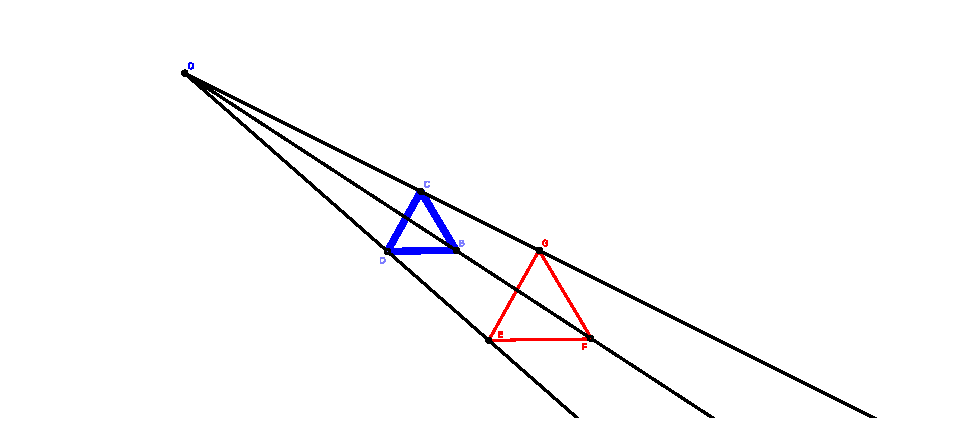
\includegraphics[width=\textwidth]{homothetie.eps}
%   \caption{Représentation graphique d'une homothétie de centre O}
%   \label{fig:homothetie}
% \end{figure}

\begin{prop}
  Soient $t$ une translation et $h$ une homothétie de rapport $\lambda$, alors
  \begin{itemize}
  \item pour tous point $A$ et $B$, si $A'=t(A)$ et si $B'=t(B)$ alors $\vect{A'B'}=\vect{AB}$. On dit que $t$ conserve les distances, $t$ est une isométrie;
  \item soient $A$ et $B$ des points, si $A'=h(A)$ et si $B'=h(B)$ alors $\vect{A'B'}=\lambda\vect{AB}$;
  \item soit $\Dr$ une droite, alors $t(\Dr)$ et $h(\Dr)$ sont des droites parallèles à $\Dr$.
  \end{itemize}
\end{prop}
\begin{proof} On ne démontre que le troisième point. $\Dr$ est la droite passant par $A$ de vecteur directeur $\vv$ et $t$ est la translation de vecteur $\vu$ alors
  \begin{equation}
    t(\Dr)=\enstq{M \in \P}{\exists N \in \Dr \quad \vect{NM}=\vu}.
  \end{equation}
Or $N \in \Dr \iff \exists \alpha \in \R \ \vect{AN}=\alpha \vv$, donc
\begin{align}
    t(\Dr)&=\enstq{M \in \P}{\exists \alpha \in \R \quad \vect{AM}-\alpha \vv=\vu}\\
    &=\enstq{M \in \P}{\exists \alpha \in \R \quad \vect{AM}=\alpha \vv+\vu}.
  \end{align}
  Comme $\vect{At(A)}=\vu$, on peut écrire que 
\begin{equation}
  t(\Dr)=\enstq{M \in \P}{\exists \alpha \in \R \quad \vect{t(A)M}=\alpha \vv}.
\end{equation}
L'ensemble $t(\Dr)$ est donc la droite passant par $t(A)$ de vecteur directeur $\vv$, donc elle est parallèle à $\Dr$.

L'application $h$ est une homothétie de centre $\Omega$ et de rapport $\lambda$, alors
\begin{align}
  h(\Dr)&=\enstq{M \in \P}{\exists N \in \Dr \quad \vect{\Omega M}=\lambda \vect{\Omega N}}\\
    &=\enstq{M \in \P}{\exists \alpha \in \R \quad \vect{\Omega M}=\lambda \vect{\Omega A}+\lambda\alpha \vv}.
\end{align}
Comme $\vect{\Omega h(A)}=\lambda \vect{\Omega A}$ on peut écrire que 
\begin{equation}
  h(\Dr)=\enstq{M \in \P}{\exists \alpha \in \R \quad \vect{h(A) M}=\lambda\alpha \vv}.
\end{equation}
L'ensemble $h(\Dr)$ est la droite passant par $h(A)$ de vecteur directeur $\vv$ ($\lambda \neq 0$) donc elle est parallèle à $\Dr$.
\end{proof}
\begin{theo}[Théorème de Thalès]
  Soient $\Dr$ et $\Dr'$ deux droites sécantes en un point $\Omega$, $A$ et $B$ deux points distincts de $\Dr$, $A'$ et $B'$ deux points distincts de $\Dr'$. Alors
  \begin{equation}
    (AA') \parallel (BB') \iff \frac{\overline{\Omega B}}{\overline{\Omega A}}=\frac{\overline{\Omega B'}}{\overline{\Omega A'}}=\frac{\overline{BB'}}{\overline{AA'}}
  \end{equation}
\end{theo}
\begin{proof}
  Soit $h$ l'homothétie de centre $\Omega$ et de rapport $\frac{\overline{\Omega B}}{\overline{\Omega A}}$, $h(A)=B$. L'image par $h$ de la droite $(AA')$ est une droite passant par $B$ et parallèle à $(AA')$.

Si $(AA')$ et $(BB')$ sont parallèles, alors la droite $(BB')$ est l'image par $h$ de la droite $(AA')$. $A' \in \Dr'$ et $A' \in (AA')$ donc $h(A') \in h(\Dr')=\Dr'$ et $h(A') \in h(AA') = (BB')$ ainsi $h(A')$ est le point d'intersection de $\Dr'$ et de $(BB')$ : $h(A')=B'$. D'où $\frac{\overline{\Omega B}}{\overline{\Omega A}}=\frac{\overline{\Omega B'}}{\overline{\Omega A'}}$.

Si $\frac{\overline{\Omega B}}{\overline{\Omega A}}=\frac{\overline{\Omega B'}}{\overline{\Omega A'}}$ alors $h(A')=B'$ d'où $h(AA')=(BB')$. Or $h(AA')$ est une droite parallèle à $(AA')$, donc $(AA')$ est parallèle à $(BB')$.
\end{proof}

\subsection{Rotations}

\begin{defdef}
  Soient $\Omega$ un point d'affixe $\omega$ et $\alpha \in \R$. La rotation de centre $\Omega$ d'angle $\alpha$ est l'application définie comme 
\begin{equation}
\fonction{R}{\P}{\P}{M}{M' \norme{\vect{\Omega M}}= \norme{\vect{\Omega M'}} \ \congru{(\vect{\Omega M},\vect{\Omega M'})}{\alpha}{2\pi}}.
\end{equation}
 Elle est représentée dans le plan complexe par $\fonction{R'}{\C}{\C}{z}{\e^{\ii \alpha}(z-\omega) + \omega}$.
\end{defdef}
\begin{prop}
  Soient des points $A$ et $B$, $r$ une rotation telle que $A'=r(A)$, $B'=r(B)$ et $A'B'=AB$. C'est une isométrie.
\end{prop}

\subsection{Similitudes}

Une similitude directe est une transformation représenté par une application de la forme $z \longmapsto az+b$ avec $a$ un complexe non nul et $b$ un complexe quelconque. Si $a=1$ alors c'est une translation de vecteur d'affixe $b$, sinon il existe un unique point fixe appelé centre noté $\Omega$. Si on note $h=h_{\Omega, \abs{a}} \ r=r_{\Omega, \Arg{a}}$ alors $s=r \circ h=h \circ r$.

En particulier, si $\abs{a}=1$ c'est une rotation, si $a \in \R$, c'est une homothétie de rapport $a$.

\begin{prop}
  Une similitude directe conserve les angles et les rapports de distances.
\end{prop}
\begin{proof}
  Soient une similitude $s : z \longmapsto az+b$ avec $a \neq 0$, les points $A_1,A_2,A_3,A_4$ tels que $A_1 \neq A_3$ et $A_2 \neq A_4$, on note avec des primes leurs images par $s$. Alors
  \begin{equation}
    \congru{(\vect{A_1 A_3};\vect{A_2 A_4})}{\Arg\left(\frac{z_4-z_2}{z_3-z_1}\right)}{2\pi},
  \end{equation}
et aussi
\begin{align}
    &\congru{(\vect{A'_1 A'_3};\vect{A'_2 A'_4})}{\Arg\left(\frac{z'_4-z'_2}{z'_3-z'_1}\right)}{2\pi}\\
    \iff&\congru{(\vect{A'_1 A'_3};\vect{A'_2 A'_4})}{\Arg\left(\frac{a(z_4-z_2)}{a(z_3-z_1)}\right)}{2\pi}\\
    \iff&\congru{(\vect{A'_1 A'_3};\vect{A'_2 A'_4})}{(\vect{A_1 A_3};\vect{A_2 A_4})}{2\pi}.
  \end{align}
  On a aussi
\begin{equation}
  \frac{A'_2A'_4}{A'_1A'_3}=\frac{\abs{z'_4-z'_2}}{\abs{z'_3-z'_1}}=\frac{\abs{z_4-z_2}}{\abs{z_3-z_1}}=\frac{A_2A_4}{A_1A_3}.
\end{equation}
\end{proof}

\begin{prop}
  Soient $[AB]$ et $[A'B']$ deux segments de longueur non nulle. Il existe une unique similitude directe $s$ telle que $s(A)=A'$ et $s(B)=B'$.
\end{prop}
